\documentclass[a4paper,utf8]{article}
\usepackage{graphicx}
\usepackage{graphicx}
\usepackage[heading,fancyhdr]{ctex}
\usepackage{amsmath,amssymb,geometry,ulem}
\usepackage{array,tabularx,tabulary,mhchem,xspace}
\usepackage{floatrow,subfig,multirow,bigstrut}
\usepackage{siunitx,booktabs,longtable,nameref}
\lineskiplimit=1pt
\lineskip=3pt
\geometry{
    top=25.4mm, 
    left=25mm, 
    right=25mm, 
    bottom=25mm,
    headsep=5.9mm,
}
\ctexset{
    chapter = {
        name = {实验,},
        beforeskip = {-23pt}
    }
}
\newcommand{\fgref}[1]{图~\ref{#1}\xspace}
\newcommand{\seqref}[1]{式~(\ref{#1})}
\newcommand{\expinfo}[6][无]{
    {\zihao{-3}\bfseries\songti
    实验名称:\uline{\hfill\mbox{#2}\hfill} \\[2.9mm]
    学\quad 号:\uline{\makebox[25mm]{#3}}\hfill
    姓\quad 名:\uline{\makebox[25mm]{#4}}\hfill
    班\quad 级:\uline{\makebox[25mm]{#5}} \\[2.9mm]
    合作者:\uline{\makebox[25mm]{#1}} \hfill
    桌\quad 号:\uline{\makebox[25mm]{}}\hfill\makebox[25mm+4em]{}\\[2.9mm]
    指导教师:\uline{\makebox[30mm]{#6}}\hfill\mbox{} \\[2.9mm]
    实验日期:\uline{\makebox[30mm]{}}\hfill\mbox{} \\[58.7mm]
    }
}%\expinfo[合作者]{实验名称}{学号}{姓名}{班级}{指导教师}
\newcommand{\pointingbox}{
    {\zihao{4}\bfseries\songti%
    实验考核\\[3mm]
    \extrarowheight=3mm
    \begin{tabularx}{150mm}{|X|X|X|X|X|}\hline
        \hfil 项目 \hfil  & \hfil 实验预习 \hfil & \hfil 实验过程 \hfil & \hfil 分析与讨论 \hfil & \hfil 总评 \hfil \\[3mm] \hline
        \hfil 评价 \hfil &  &  &  &  \\[3mm] \hline
    \end{tabularx}
    }
}
\newcommand{\derivative}[2]{\frac{\mathrm{d} #1}{\mathrm{d} #2}}
\newcommand{\thinking}[2]{\textbf{#1}\\
答:\begin{minipage}[t]{0.85\textwidth}
    #2
\end{minipage}}

\pagestyle{fancy}
\fancyhf{}
%\fancyhead[C]{材料科学基础实验}
%\fancyfoot[C]{\thepage}
\fancyhead[EC]{\leftmark} \fancyhead[OC]{\rightmark}
\fancyhead[EL,OR]{\thepage}
\fancypagestyle{plain}{\renewcommand{\headrulewidth}{0pt}\fancyhf{}}

\newcounter{Rownumber}
\newcommand*{\Rown}{\stepcounter{Rownumber}\theRownumber}
\newcounter{sample}
\newcommand*{\Sam}{\stepcounter{sample}\thesample}
\newcounter{Fignumber}
\newcommand*{\Fign}{\stepcounter{Fignumber}\theFignumber}

\newcommand*{\resetRown}{\setcounter{Rownumber}{0}}
\newcommand{\qrange}[3]{\qtyrange[range-phrase = \text{$\sim$},range-units =single]{#1}{#2}{#3}}
\floatsetup[table]{capposition=top}
\newcolumntype{C}{>{\hfil}X<{\hfil}}
\renewcommand{\Nameref}[1]{\textbf{\ref{#1}~\nameref{#1}}}
\newcommand{\TTR}[0]{\watt\per\m\per\K}
\graphicspath{{img/}}
\begin{document}
\begin{center}
    {\mbox{}\\[7em]\zihao{2}\bfseries\songti%
    材料科学基础实验预习报告}\\[34mm]
    \expinfo{四探针法测量半导体电阻率和薄层电阻}{22301056}{王俊杰}{22 材物}{艾斌}
\end{center}
\newpage
\section{实验目的}
    \begin{enumerate}
        \item 理解四探针方法测量半导体电阻率和薄层电阻的原理;
        \item 学会用四探针方法测量半导体电阻率和薄层电阻;
        \item 针对不同几何尺寸的样品,了解其修正方法;
        \item 了解影响测量结果准确性的因素及避免方法
    \end{enumerate}
\section{实验原理}%简单描述,含必要的公式和附图;
    \subsection{半导体材料体电阻率的测量}
        \subsubsection{半无穷大样品体电阻率的测量}
            在电阻率分布均匀的半无穷大样品表面上,若电流 I 通过探针以点电流源的形式注入到半导体材料内部,则电流密度在材料内部是均匀分布的,具体是以探针尖为球心沿径向放射状分布。四探针法测量半导体材料体电阻率采用四根金属探针排成一列,并且四根金属探针的间距相等,均为 $S$。将四根金属探针压在一块半无穷大的半导体材料表面上,当 1、4 探针通以电流 $I$(探针 1 为正极,探针 4 为负极),2、3 探针上测得的电压为 $V_{23}$ 时,只要样品厚度及边缘与探针的最近距离大于四倍探针间距,半无穷大样品的体电阻率 $\rho$ 可表示为:
            \begin{equation}
                \rho = 2\pi S\cdot\frac{V_{23}}{I} \label{eq:0}
            \end{equation}
            半导体材料的电阻率对温度比较灵敏,因此,测试半导体材料的电阻率时不但要记录测试的环境温度,还要将该温度下的实测电阻率修正到 23℃下的电阻率,引入修正系数 $F_T$ : 
            \begin{equation}
                \rho =\frac{2\pi S}{F_T}\cdot\frac{V_{23}}{I}
            \end{equation}
            \begin{figure}[!ht]
                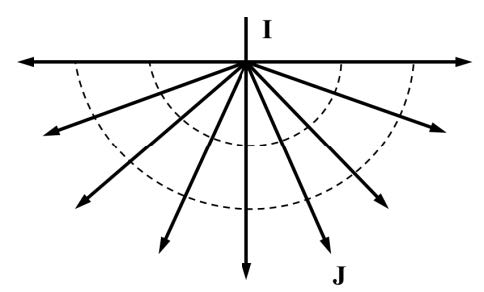
\includegraphics[width=0.4\textwidth]{1.jpg}
                \caption{电流 $I$ 以点接触的形式注入到半无穷大样品内部的电流密度分布}
            \end{figure}
        \subsubsection{无穷大薄样品体电阻率的测量}
            类似前面的分析,无穷大薄样品的体电阻率 $\rho$ 可表示为:
            \begin{equation}
                \rho =\frac{\pi V_{23}}{I \ln 2} \label{eq:1}
            \end{equation}
    \subsection{半导体材料电阻的测量}        
        \subsubsection{半导体薄层电阻(或方块电阻)的测量}
            如果扩散片的结深用 $X_j$ 表示,根据定义,方块电阻 $R_{sq}$ 可表示为:
            \begin{equation}
                R_{sq}=\rho\frac{L}{L\cdot X_{j}}=\frac{\rho}{X_{j}} \label{eq:2}
            \end{equation}
            将 \seqref{eq:1} 代入 \seqref{eq:2} 得:
            \begin{equation}
                R_{sq}=4.5324\frac{V_{23} d}{I} \label{eq:3}
            \end{equation}
            实际测量中,只要薄层的厚度小于 $0.5S$,并且样品面积相对于探针间距 $S$ 可视为无穷大时,就可以利用\seqref{eq:3}计算薄层电阻。如果不能将样品的横向面积视为无穷大,也需要使用包含修正因子 $F$ 的公式来计算方块电阻:
            \begin{equation}
                R_{sq}= F \frac{V_{23}}{I} \label{eq:4}
            \end{equation}
        
\section{实验仪器}%规格及参数
    KDY-1 型四探针电阻率/方阻测试仪,一台计算机;p 型单晶硅棒(电阻率样品)、p 型单晶硅片(薄样品)、p 型硅基底上的 n 型扩散片(薄层电阻样品)各一个
\section{实验过程}%简述主要过程和实验内容
    \subsection{测量样品电阻率或方块电阻的操作步骤}
    \begin{enumerate}
        \item 打开 KDB-1 四探针测试仪后面板上的电源开关,此时恒流源已开启,测试电流自动处于 \SI{1}{\milli\ampere} 档。根据测试目的,将测试仪后面板上的 “电阻率/方块电阻测试切换开关”($\rho/R$ 开关)拨到相应位置。
        \item 将样品置于样品台上,旋转测试架上的手轮使探针下降,同时调整样品位置,使四根探针正好落在样品的测试点。当探针快要接触样品时,应缓慢旋转手轮,使探针缓慢轻压在样品上。当听到主机传来“咔嗒”一声、且前面板左侧的两块绿字电表有数值显示,即表示探针与样品已接触到位,应立即停止旋转手轮。
        \item 根据附表给出的推荐值,并通过选择合适的测试电流档位和恒流源电压档位,调节测试电流和恒流源电压旋钮,使测试电流达到合适的值,此时,电压表显示的 $V_{23}$ 应出现尽可能多的有效数字,且电压值在测试电流不变的前提下能长时间保持稳定,而且正测和反测得到的 $V_{23}$ 的绝对值差别也不大。
        \item 记录此时的测试电流 I 和电压 $V_{23}$ 的值,由相应公式计算样品的电阻率或方块电阻。测量完毕,升起探针,取走样品。
    \end{enumerate}
    \subsection{测量 p 型硅棒的电阻率}
        使用厂家推荐的测试电流对硅棒横截面上五个不同位置处(中心点和距离圆心 1/3 半径处的 4 个等距点)的电阻率进行测量。为了减小测量误差,对同一点的测量分别进行正向和反向测量。将实验结果记录到表中,使用\seqref{eq:0} 计算电阻率 $\rho (T)$。利用附录将测得的电阻率修正到 \SI{23}{\degreeCelsius}。此外,利用下面的公式计算电阻率分布的不均匀度。
    \subsection{测量 p 型单晶硅片(薄样品)的电阻率}
        \begin{enumerate}
            \item 直读法,根据样品厚度和附表 4 得到直读电流的值,并将其设置为测试电流,直接
            从电压表上读取样品的电阻率。
            \item 选择合适的测试电流 $I$ 和测得的电压 $V_{23}$,采用 $\rho(T)=\frac{V_{23}}l\cdot d\cdot F_{SP}\cdot F(d/S)\cdot F(S/D)$ 计算硅片的电阻率。对硅片中心位置处的电阻率测量 5 次。每次测量完毕后,升起探针,将硅片逆时针旋转 $\SI{30}{\degree} \sim  \SI{35}{\degree}$ 进行下一次测量。同一位置正向和反向各测量一次,并将测量结果修正到 \SI{23}{\degreeCelsius}。
        \end{enumerate}
    \subsection{测量 p 型单晶硅衬底上的 n 型扩散片的方块电阻}
        扩散片的结深 $X_j$ 和尺寸由老师现场提供。由于待测扩散片近似正方形,故取最短的边长作为扩散片的直径 $D$ 。将探针压在扩散片的中心位置进行方块电阻的测量。
        \begin{enumerate}
            \item 直读法,设置合适的测试电流,从电压表上直接读出样品的方块电阻。
            \item 根据测试电流、电压 $V_{23}$ 以及扩散片的尺寸,利用\seqref{eq:4}计算扩散片的方块电阻。需要测量两个位置的方块电阻,即在第一次测量完成之后将样品旋转 \SI{90}{\degree} 再测量一次。同一位置正向和反向各测量一次。
        \end{enumerate}
    \subsection{测量两种透明导电玻璃的方块电阻}
        本实验提供两种透明导电玻璃(FTO 导电玻璃和 ITO 玻璃),测试方法及要求与测试扩散片一致。
        \pagebreak
\section{实验数据与分析}
    \subsection{实验数据}
        \begin{table}[!ht]
            \caption{p 型硅棒的电阻率实验数据}
            \zihao{-5}
            \begin{tabular}{*{6}{c}}
                \toprule
                \multicolumn{2}{c}{温度/\unit{\degreeCelsius}} & \multicolumn{2}{c}{样品厚度/\unit{\mm}} & \multicolumn{2}{c}{样品直径/\unit{\mm}} \\
                \multicolumn{2}{c}{21.7} & \multicolumn{2}{c}{25} & \multicolumn{2}{c}{24} \\ \midrule
                位置 & 测试电流/\unit{\mA} & 正向电压/\unit{\mV} & 反向电压/\unit{\mV} & 电阻率 $\rho_T$/\unit{\ohm\cm} & 电阻率$\rho_{23}$/\unit{\ohm\cm} \\
                \Rown & 0.5893 & 1.57 & 1.57 & 1.67 & 1.68 \\
                \Rown & 0.5893 & 1.55 & 1.56 & 1.65 & 1.67 \\
                \Rown & 0.5893 & 1.57 & 1.56 & 1.66 & 1.68 \\
                \Rown & 0.5893 & 1.60 & 1.60 & 1.70 & 1.72 \\
                \Rown & 0.5893 & 1.58 & 1.59 & 1.68 & 1.70 \\ \midrule
                \multicolumn{3}{c}{电阻率 $\rho_T$ 平均值/\unit{\ohm\cm}} & \multicolumn{3}{c}{电阻率 $\rho_T$ 不均匀度} \\
                \multicolumn{3}{c}{1.68} & \multicolumn{3}{c}{$2.85\%$} \\ \bottomrule
            \end{tabular}
        \end{table}\par
        \setcounter{Rownumber}{0}
        \begin{table}[!ht]
            \caption{p 型单晶硅片(薄样品)的电阻率}
            \zihao{-5}
            \begin{tabular}{*{6}{c}}
                \toprule
                温度/\unit{\degreeCelsius} & 样品厚度/\unit{\mm} & 样品直径/\unit{\mm} & $F(d/S)$ & $F(S/D)$ & $F_{sp}$ \\
                21.7 & 0.4 & 76.2 & 0.9993 & 4.525 & 1 \\ \midrule
                \multirow{2}{*}{直读法} & \multicolumn{2}{c}{测试电流/\unit{\mA}} & \multicolumn{3}{c}{直读电阻率/\unit{\ohm\cm}} \\
                 & \multicolumn{2}{c}{0.1811} & \multicolumn{3}{c}{18.32} \\ \midrule
                测量 & 测试电流/\unit{\mA} & 正向电压/\unit{\mV} & 反向电压/\unit{\mV} & 电阻率 $\rho_T$/\unit{\ohm\cm} & 电阻率$\rho_{23}$/\unit{\ohm\cm} \\
                \Rown & 0.8892 & 89.96 & 89.93 & 18.29 & 18.47 \\
                \Rown & 0.8828 & 89.58 & 89.86 & 18.38 & 18.55 \\
                \Rown & 0.8751 & 88.76 & 88.85 & 18.35 & 18.53 \\
                \Rown & 0.8605 & 87.10 & 87.15 & 18.31 & 18.48 \\
                \Rown & 0.7940 & 80.50 & 80.60 & 18.35 & 18.52 \\ \midrule
                \multicolumn{6}{c}{电阻率 $\rho_T$ 平均值/\unit{\ohm\cm}} \\
                \multicolumn{6}{c}{18.34} \\ \bottomrule
            \end{tabular}
        \end{table}\par
        \setcounter{Rownumber}{0}
        \begin{table}[!ht]
            \caption{p 型单晶硅衬底上的 n 型扩散片的方块电阻}
            \zihao{-5}
            \begin{tabular}{*{6}{c}}
                \toprule
                温度/\unit{\degreeCelsius} & 样品结深/\unit{\mm} & 样品直径/\unit{\mm} & $F(d/S)$ & $F(S/D)$ & $F_{sp}$ \\
                23 & 0.001 & 75 & 1 & 4.525 & 1 \\ \midrule
                \multirow{2}{*}{直读法} & \multicolumn{2}{c}{测试电流/\unit{\mA}} & \multicolumn{3}{c}{直读电阻率/\unit{\ohm\cm}} \\
                 & \multicolumn{2}{c}{4.532} & \multicolumn{3}{c}{18.32} \\ \midrule
                测量 & 测试电流/\unit{\mA} & 正向电压/\unit{\mV} & 反向电压/\unit{\mV} & \multicolumn{2}{c}{方块电阻/$\unit{\ohm}\cdot \square$} \\
                \Rown & 4.915 & 78.23 & 78.72 & \multicolumn{2}{c}{72.25} \\
                \Rown & 4.842 & 76.82 & 75.40 & \multicolumn{2}{c}{71.13} \\ \midrule
                \multicolumn{6}{c}{方块电阻平均值/$\unit{\ohm}\cdot \square$} \\
                \multicolumn{6}{c}{71.69} \\ \bottomrule
            \end{tabular}
        \end{table}\par
        \setcounter{Rownumber}{0}
        \begin{table}[!ht]
            \caption{FTO 玻璃方块电阻}
            \zihao{-5}
            \begin{tabular}{*{6}{c}}
                \toprule
                温度/\unit{\degreeCelsius} & 薄膜厚度/\unit{\um} & 样品直径/\unit{\mm} & $F(d/S)$ & $F(S/D)$ & $F_{sp}$ \\
                23 & 0.185 & 75 & 1 & 4.521 & 1 \\ \midrule
                \multirow{2}{*}{直读法} & \multicolumn{2}{c}{测试电流/\unit{\mA}} & \multicolumn{3}{c}{直读电阻率/\unit{\ohm\cm}} \\
                 & \multicolumn{2}{c}{4.532} & \multicolumn{3}{c}{7.37} \\ \midrule
                测量 & 测试电流/\unit{\mA} & 正向电压/\unit{\mV} & 反向电压/\unit{\mV} & \multicolumn{2}{c}{方块电阻/$\unit{\ohm}\cdot \square$} \\
                \Rown & 4.853 & 7.90 & 7.90 & \multicolumn{2}{c}{7.36} \\
                \Rown & 5.036 & 8.25 & 8.25 & \multicolumn{2}{c}{7.41} \\ \midrule
                \multicolumn{6}{c}{方块电阻平均值/$\unit{\ohm}\cdot \square$} \\
                \multicolumn{6}{c}{7.38} \\ \bottomrule
            \end{tabular}
        \end{table}\par
        \setcounter{Rownumber}{0}
        \begin{table}[!ht]
            \caption{ITO 玻璃方块电阻}
            \zihao{-5}
            \begin{tabular}{*{6}{c}}
                \toprule
                温度/\unit{\degreeCelsius} & 薄膜厚度/\unit{\um} & 样品直径/\unit{\mm} & $F(d/S)$ & $F(S/D)$ & $F_{sp}$ \\
                23 & 1.2 & 75 & 1 & 4.521 & 1 \\ \midrule
                \multirow{2}{*}{直读法} & \multicolumn{2}{c}{测试电流/\unit{\mA}} & \multicolumn{3}{c}{直读电阻率/\unit{\ohm\cm}} \\
                 & \multicolumn{2}{c}{4.532} & \multicolumn{3}{c}{2.20} \\ \midrule
                测量 & 测试电流/\unit{\mA} & 正向电压/\unit{\mV} & 反向电压/\unit{\mV} & \multicolumn{2}{c}{方块电阻/$\unit{\ohm}\cdot \square$} \\
                \Rown & 2.907 & 0.91 & 0.91 & \multicolumn{2}{c}{1.42} \\
                \Rown & 3.339 & 1.04 & 1.04 & \multicolumn{2}{c}{1.41} \\ \midrule
                \multicolumn{6}{c}{方块电阻平均值/$\unit{\ohm}\cdot \square$} \\
                \multicolumn{6}{c}{1.41} \\ \bottomrule
            \end{tabular}
        \end{table}\par
        %\clearpage
        \subsection{不确定度分析}
    \subsubsection{A 类不确定度分量的评估}
    对一个随机变量 $x$ 进行了 $n$ 次重复测量,其算术平均值 $\bar{x}$ 作为对被测量 $x$ 的最佳统计评估值,平均值的标准偏差 $s(\bar{x})$ 作为实验结果的标准不确定度,自由度 $\nu=n-1$。计算公式为\\
    \begin{align}
        \bar{x}&=\frac{1}{n}\sum_{i=1}^{n}x_i \label{exp:amean} \\
        s(\bar{x})&=\sqrt{\frac{1}{n(n-1)}\sum_{i=1}^{n}(x_i-\bar{x})^2} \label{exp:astd}
    \end{align}

    \subsubsection{B 类不确定度分量的评估}
    对一个非重复测量得到的量 x 进行不确定度分析时,评估者需根据已获得的信息人为假定其服从某种概率分布来评估其方差 $u^2(x)$ 或标准不确定度 $u(x)$。具体步骤是,首先根据量 $x$ 的变化范围确定其半宽度 $a$,然后根据假定的概率分布计算标准不确定度。\\
    \begin{equation}
        u(x) = \frac a k \label{exp:uncertaintyB}
    \end{equation}
    在 100\% 和 95\% 置信概率下,矩形分布时的包含因子 $k$ 值分别为 $\sqrt{3}$ 和 $1.65$,三角形分布时的包含因子 $k$ 值分别为 $\sqrt{6}$ 和 $1.90$,正态分布时的包含因子 $k$ 值分别为 $3$ 和 $1.96$。

    \subsubsection{直接测量量的合成标准不确定度}
    直接测量量的合成标准不确定度 $u_c(x)$ 由其 A 类标准不确定度分量 $s(\bar{x})$ 与其 B 类标准不确定度分量 $u(x)$ 采用方和根法合成,即\\
    \begin{equation}
        u_c(x) = \sqrt{s^2(\bar{x})+u^2(x)} \label{exp:uncertaintyCombine}
    \end{equation}
    合成标准不确定度 $u_c$ 的自由度称为有效自由度,用 $\nu_\text{eff}$ 表示。当各分量间相互独立且合成量接近正态分布或 t 分布时,有效自由度 $\nu_\text{eff}$ 可以由下面的韦尔奇-萨特韦特(Welch-Satterthwaite)公式计算\\
    \begin{equation}
        \nu_\text{eff}=\frac{u_c^4(x)}{\displaystyle\frac{s^4(x)}{\nu_\text{A}}+\frac{u^4(x)}{\nu_\text{B}}} \label{exp:validFreedom}
    \end{equation}
    式中 $\nu_\text{A}$ 和 $\nu_\text{B}$ 分别是 A 类和 B 类标准不确定度分量对应的自由度数。如果 $\nu_\text{eff}$ 不是整数,则去掉小数部分取整,即将 $\nu_\text{eff}$ 取为一个不大于 $\nu_\text{eff}$ 本身的整数。

    \subsubsection{标准不确定度的传播规律}
    标准不确定度传播规律的数学基础是全微分。假设间接测量量 $y$ 与直接测量量 $x_1$, $x_2$, $x_3$, $\cdots$, $x_n$ 满足函数关系 $y = f(x_1,x_2,x_3,\cdots,x_n)$,且各个直接测量量 $x_1$, $x_2$, $x_3$, $\cdots$, $x_n$ 是相互独立的。对于以标准偏差表示的标准不确定度,需以方和根的形式求和,因此,当各个直接测量量依次有 $u(x_1)$, $u(x_2)$, $u(x_3)$, $\cdots$, $x_n$ 的标准不确定度时,间接测量量 $y$ 的标准不确定度 $u_c(y)$ 可以表示为\\
    \begin{equation}
        u_c^2(y)=\sum_{i=1}^{n}\left[\frac{\partial f}{\partial x_i}\right]^{2}u^2\left(x_{i}\right)=\sum_{i=1}^{n}c_i^2 u^2\left(x_{i}\right) \label{exp:uncertaintyPropagation}
    \end{equation}
    间接测量量 $y$ 的有效自由度由下式计算\\
    \begin{equation}
        \nu_\text{eff}=\frac{u_c^4(y)}{\displaystyle\sum_{i=1}^{n}\frac{c_i u^4(x_i)}{\nu_i}} \label{exp:validFreedom2}
    \end{equation}

    当需要评定扩展不确定度 $U$ 时,可根据合成标准不确定度的有效自由度 $\nu_\text{eff}$ 和给定的置信概率(譬如 95\%),通过查 t 分布表得出包含因子 $k$,进而给出扩展不确定度 $U = k u_c$。

        \subsection{对 p 型单晶硅片(薄样品)的电阻率不确定度的计算}
        \subsubsection{仪器引入的标准不确定度}
        不确定度主要来源为恒流源,数字电压表与硅片厚度测量结果。已知数字电压表的测试量程为  \qrange{0.2}{50}{\mV},分辨率优于 $\pm 0.05 \% $。在 $1 \unit{\mA}$ 电流档,恒流源最大允许误差为 $\pm 0.02 \unit{\mA}$;在 $10 \unit{\mA}$ 电流档,恒流源最大允许误差为 $ \pm 0.1 \unit{\mA} $ 。硅片厚度测量结果的相对不确定为 $ \pm 0.2\% $。探针间距修正因子 $ F_{sp}$、样品厚度修正因子 $F(d/S)$和直径修正因子 $ F(S/D) $ 引入的不确定度可以忽略。假定矩形分布来评估仪器精度引入的不确定度。利用\seqref{exp:uncertaintyB},取 $k=\sqrt{3}$,可得: \par
        \begin{table}[!ht]
            \caption{仪器的不确定度}
            \centering\begin{tabular}{c c c}\toprule
                直接测量量 & 精度 & B 类不确定度 \\ \midrule
                \makebox[50mm]{数字电压表} & $\pm\SI{0.025}{\mV}$ &\makebox[50mm]{\SI{0.015}{\mV}} \\
                恒流源(1 \unit{\mA} 档) & $ \pm\SI{0.02}{\mA}$ & \SI{0.012}{\mA} \\
                恒流源(10 \unit{\mA} 档) & $ \pm\SI{0.1}{\mV}$ & \SI{0.058}{\mV} \\
                硅片厚度 &  & 0.2\% \\ \bottomrule
            \end{tabular}
        \end{table}
        \subsubsection{数学模型}
        硅片电阻率的测量结果由下式给出
        \begin{align}
            \rho_i &= \frac{V_i}{I_i}\cdot d\cdot F_{sp}\cdot F(d/S)\cdot F(S/D) \\
            \bar{\rho} &= \frac{1}{5} \sum_{i=1}^5 \rho_i
        \end{align}
        \subsubsection{有贡献的方差}
        ,假设 $\rho_i$ 服从正态分布,利用\seqref{exp:uncertaintyPropagation} 可得
        \begin{align}
            u^2(\rho_i) &= c^2_{Vi} u^2(V_i)+c^2_{Ii} u^2(I_i)+c^2_{d} u^2(d) \\
            u^2(\bar{\rho}) &= \frac{1}{5 (5-1)} \sum_{i=1}^{5}(\rho_i-\bar{\rho})^2 \label{exp:18}\\
            u_c^2(\rho) &= \frac{1}{5^5} \sum_{i=1}^{5}u^2(\rho_i)+s^2(\bar{\rho}) \label{exp:17}
        \end{align}
        其中,\\
        $c_V=\partial \rho_i / \partial V_i=1/I_i\cdot d\cdot F$ \\
        $c_I=\partial \rho_i / \partial I_i=-V_i/I_i^2\cdot d\cdot F$ \\
        $c_d=\partial \rho_i / \partial d=V_i/I_i\cdot F$\\
        式中 $F=F_{SP}\cdot F(d/S)\cdot F(S/D)/F_T=4.56522$,由矩形分布得
        \begin{align}
            V_i &= \frac{V_{i1}+V_{i2}}{2}\\
            u^2(V_i) &= \frac{1}{12} (a^2+a^2) = \frac{a^2}{6} = \frac{u^2(V)}{2}
        \end{align}
        其中 $a$ 为电压表的精度,计算得 $u(\bar{\rho})=0.000242958$ 和表 \ref{table:7}
        \setcounter{Rownumber}{0}
        \begin{table}[!ht]
            \caption{硅片电阻率的测量结果的 B 类不确定度}\label{table:7}
            \begin{tabular}{ccccc}\toprule
                \makebox[15mm]{$i$} & \makebox[20mm]{$|c_{Vi}|$} & \makebox[20mm]{$|c_{Ii}|$} & \makebox[20mm]{$|c_{d}|$} & \makebox[20mm]{$u(\rho_i)/\unit{\ohm\per\cm}$} \\ \midrule
                \Rown & 0.205363 & 20.7730 & 461.785 & 0.240822 \\
                \Rown & 0.206852 & 21.0226 & 463.969 & 0.243701 \\
                \Rown & 0.208672 & 21.1760 & 463.278 & 0.245463 \\
                \Rown & 0.212213 & 21.4864 & 462.225 & 0.249029 \\
                \Rown & 0.229986 & 23.3317 & 463.134 & 0.270269 \\ \bottomrule
            \end{tabular}
        \end{table}
        \subsubsection{合成标准不确定度}
        代入\seqref{exp:17} 和\seqref{exp:18}得
        \begin{equation}
            u_c^2(\rho)=\frac{1}{5^5} \sum_{i=1}^{5}u^2(\rho_i) + u^2(\bar{\rho})= 0.01275~\unit{\ohm^2\cm^{-2}}
        \end{equation}
        或
        \begin{equation}
            u_c(\rho)=0.12~\unit{\ohm\per\cm}
        \end{equation}
        相对不确定度为
        \begin{equation}
            \frac{u_c(\rho)}{\rho}=\frac{0.12}{18.34} = 6.2 \times 10^{-3}
        \end{equation}
        \subsubsection{扩展不确定度}
        包含因子 $k = 2$,可得
        \begin{equation}
            U=k u_c(\rho)=0.23~\unit{\ohm\per\cm}
        \end{equation}\par
        最终结果可表示为
        \begin{equation}
            \rho_T = (18.34 \pm 0.23)~\unit{\ohm\per\cm}
        \end{equation}
\section{结果分析与讨论}
    从测量 p 型硅棒的电阻率实验数据可以看出,考虑测量误差的情况下,硅棒横截面上五个位置处的电阻率仍然有3\%以上的不均匀度。而 p 型单晶硅片(薄样品)的电阻率测量的相对误差很小,精确度高。
\section{思考题} 
    \subsection{电阻率和方块电阻的测量结果的误差来源有哪些?应如何避免?}
        \begin{enumerate}
            \item 仪器的测量精度导致的误差;难以消除,只能使用更精确的仪器。
            \item 每次测量的随机误差;多次测量取平均值。
            \item 测量条件的不完全一致导致的误差;尽可能保证在相同环境下进行实验。
        \end{enumerate}
    \subsection{影响测量结果准确性的外界因素有哪些?应如何避免?}
        \begin{enumerate}
            \item 污渍;由于样品的重复使用,样品上的杂质也会影响测试结果,可以先用清洁再测试。
            \item 温度;晶格的震动强度与温度相关,因此半导体材料的电阻率对温度敏感,所以应该恒温下进行测试。
        \end{enumerate}
\end{document}